\documentclass{article}
\usepackage{graphicx}
\graphicspath{ {images/} }

\title{Moeda White Paper}
\author{Taynaah Reis}
\date{July 2017}


\begin{document}

\maketitle

\section{Introduction}

MOEDA is a Cooperative Crypto Impact Investment Banking-as-a-Service Platform designed to:

- Provide Community-focused mobile lending system

- Provide a multi-purpose digital identity and opportunities to build creditworthiness and reputation

- Give investors real-time transparency of SDG-aligned Impact Investment and trust of cryptographically assured blockchain records and contracts

- Facilitate to efficiently scale community investments, payment transactions and service more customers online

MOEDA (“coin” in Portuguese) began as a hackathon submission for the Blockchain SDG Hackathon at IMPACT CONVERGENCE 2.0. The team developed an idea that demonstrated how blockchain technology can be utilized towards United Nations SDGs (Sustainable Development Goals.). The submission was selected as the winner and invited to present to a global audience at United Nations ECOSOC Chamber. 

\begin{figure}[h]
    \centering
    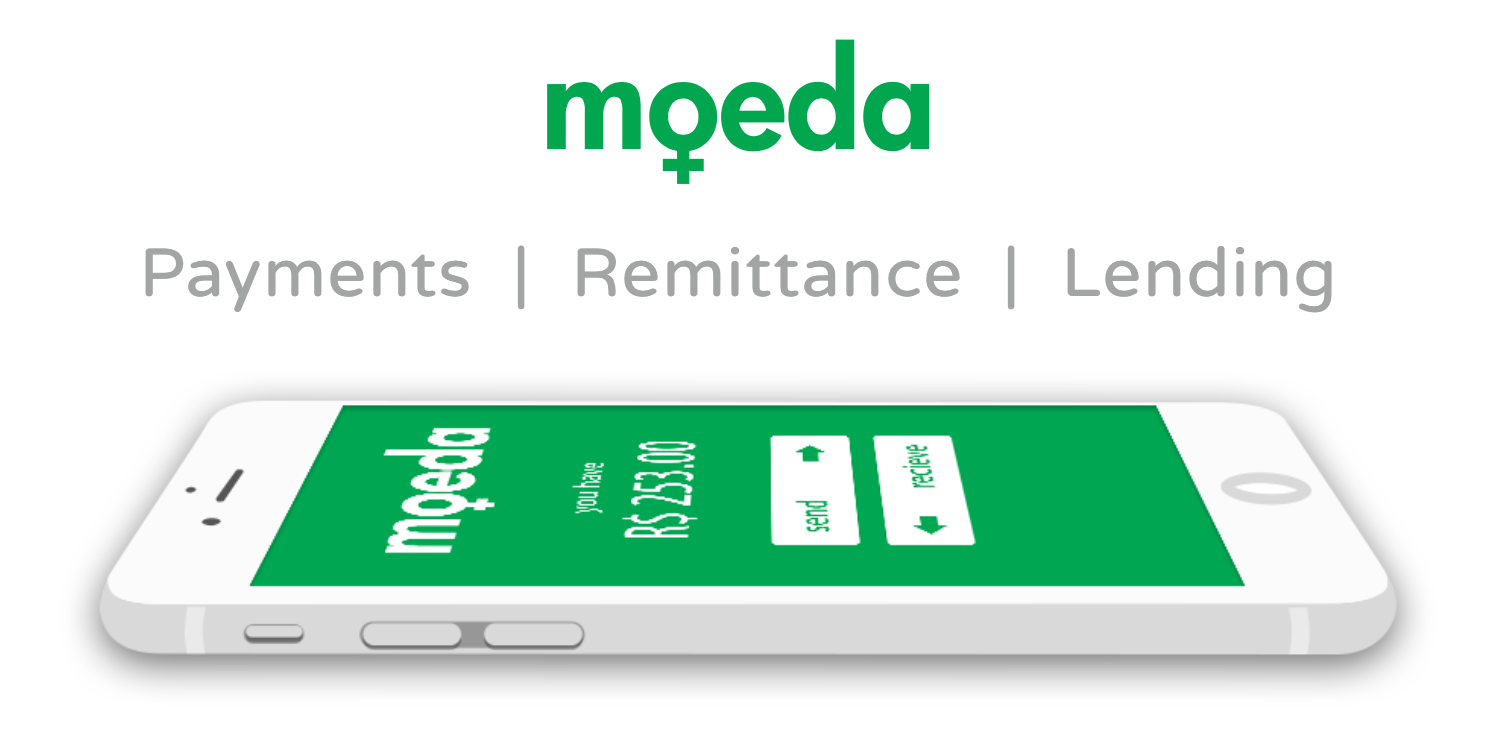
\includegraphics[width=10cm,keepaspectratio,]{mda}
   
\end{figure}

\section{MOEDA Cooperative Crypto Banking}

\subsection{Cooperative Banking}

According to the World Bank, approximately 2 billion people of the world are not included on the financial system, don’t have access to a banking account, or worse, they have negative credit and are in debt. 

Across the globe, credit cooperatives aim to service many of these underbanked individuals. 

The next most viable market, China, has 300 million farmers, 32,000 + rural credit cooperatives who could also benefit from participating in a platform like MOEDA.

MOEDA is organized on a cooperative basis to the people, by the people and from the people.

The Cooperative Banking involves decentralized autonomous association of people united voluntarily to meet their common economic, social and cultural needs through a jointly owned and democratically controlled enterprise.


\subsection{Free-Trade Zone}

To achieve MOEDA’s mission of connecting disadvantaged entrepreneurs to modern financial systems we aim to license our proprietary technologies and operate our cooperative banking services in a global scale. That’s why we have established MOEDA’s Holding Technology Co. company in Uruguay free-trade zone, a special economic zone part of the Latin America Free Trade Association (LAFTA).

``Uruguay's free-trade zone gives us the operational flexibility to straddle the real world and the digital world," says MOEDA co-founder Taynaah Reis. ``We are encouraged by the Uruguayan government’s business-friendly environment and we have many advantages, including tax exemptions, unfettered foreign currency trading and logistical support."

Also, the introduction and trade of foreign currency, gold, precious metals, and public values, is completely free. Payment and collection of commercial transactions does not require the intervention of any economic authority, including the Central Bank of Uruguay.

Like in the rest of the Uruguayan territory, there is no exchange control, inflow and outflow of foreign currency is free. 

U.S. investment bank Merrill Lynch, India’s Tata Consulting and copier maker Ricoh are among international companies that have established operations in Uruguay’s free-trade zones, according to published reports.

Moeda plans to maximize its use by being established in free-trade zones in Uruguay and other countries to improve the overall trade efficiency of its clients and partner organizations.


\subsection{Cooperative Principles}
Moeda is aligned with the principles of the World Council of Credit Unions (WOCCU). The leading international trade association and development agency for credit unions and cooperative financial institutions. The World Council promotes the self-sustainable development of credit unions and other financial cooperatives around the world to empower people through access to high quality and affordable financial services.

Principles:

o	Institutional development and self-sufficiency

o	Market based approaches to savings mobilization

o	Increasing access to financial services through democratic participation

o	Loan services emphasizing member needs and high repayment rates

o	Safety and efficiency through financial management systems and controls

o	Assistance in developing an effective legal/regulatory framework

o	International exchange among credit unions through partnerships

o	Micro-enterprise through access to savings and credit services

o	Support of women through awareness of gender issues. 

\subsection {Roadmap}

Moeda has a goal-oriented roadmap. We aim to significantly improve people lives, by funneling sustainable development investments to their communities.

\begin{figure}[h]
    \centering
    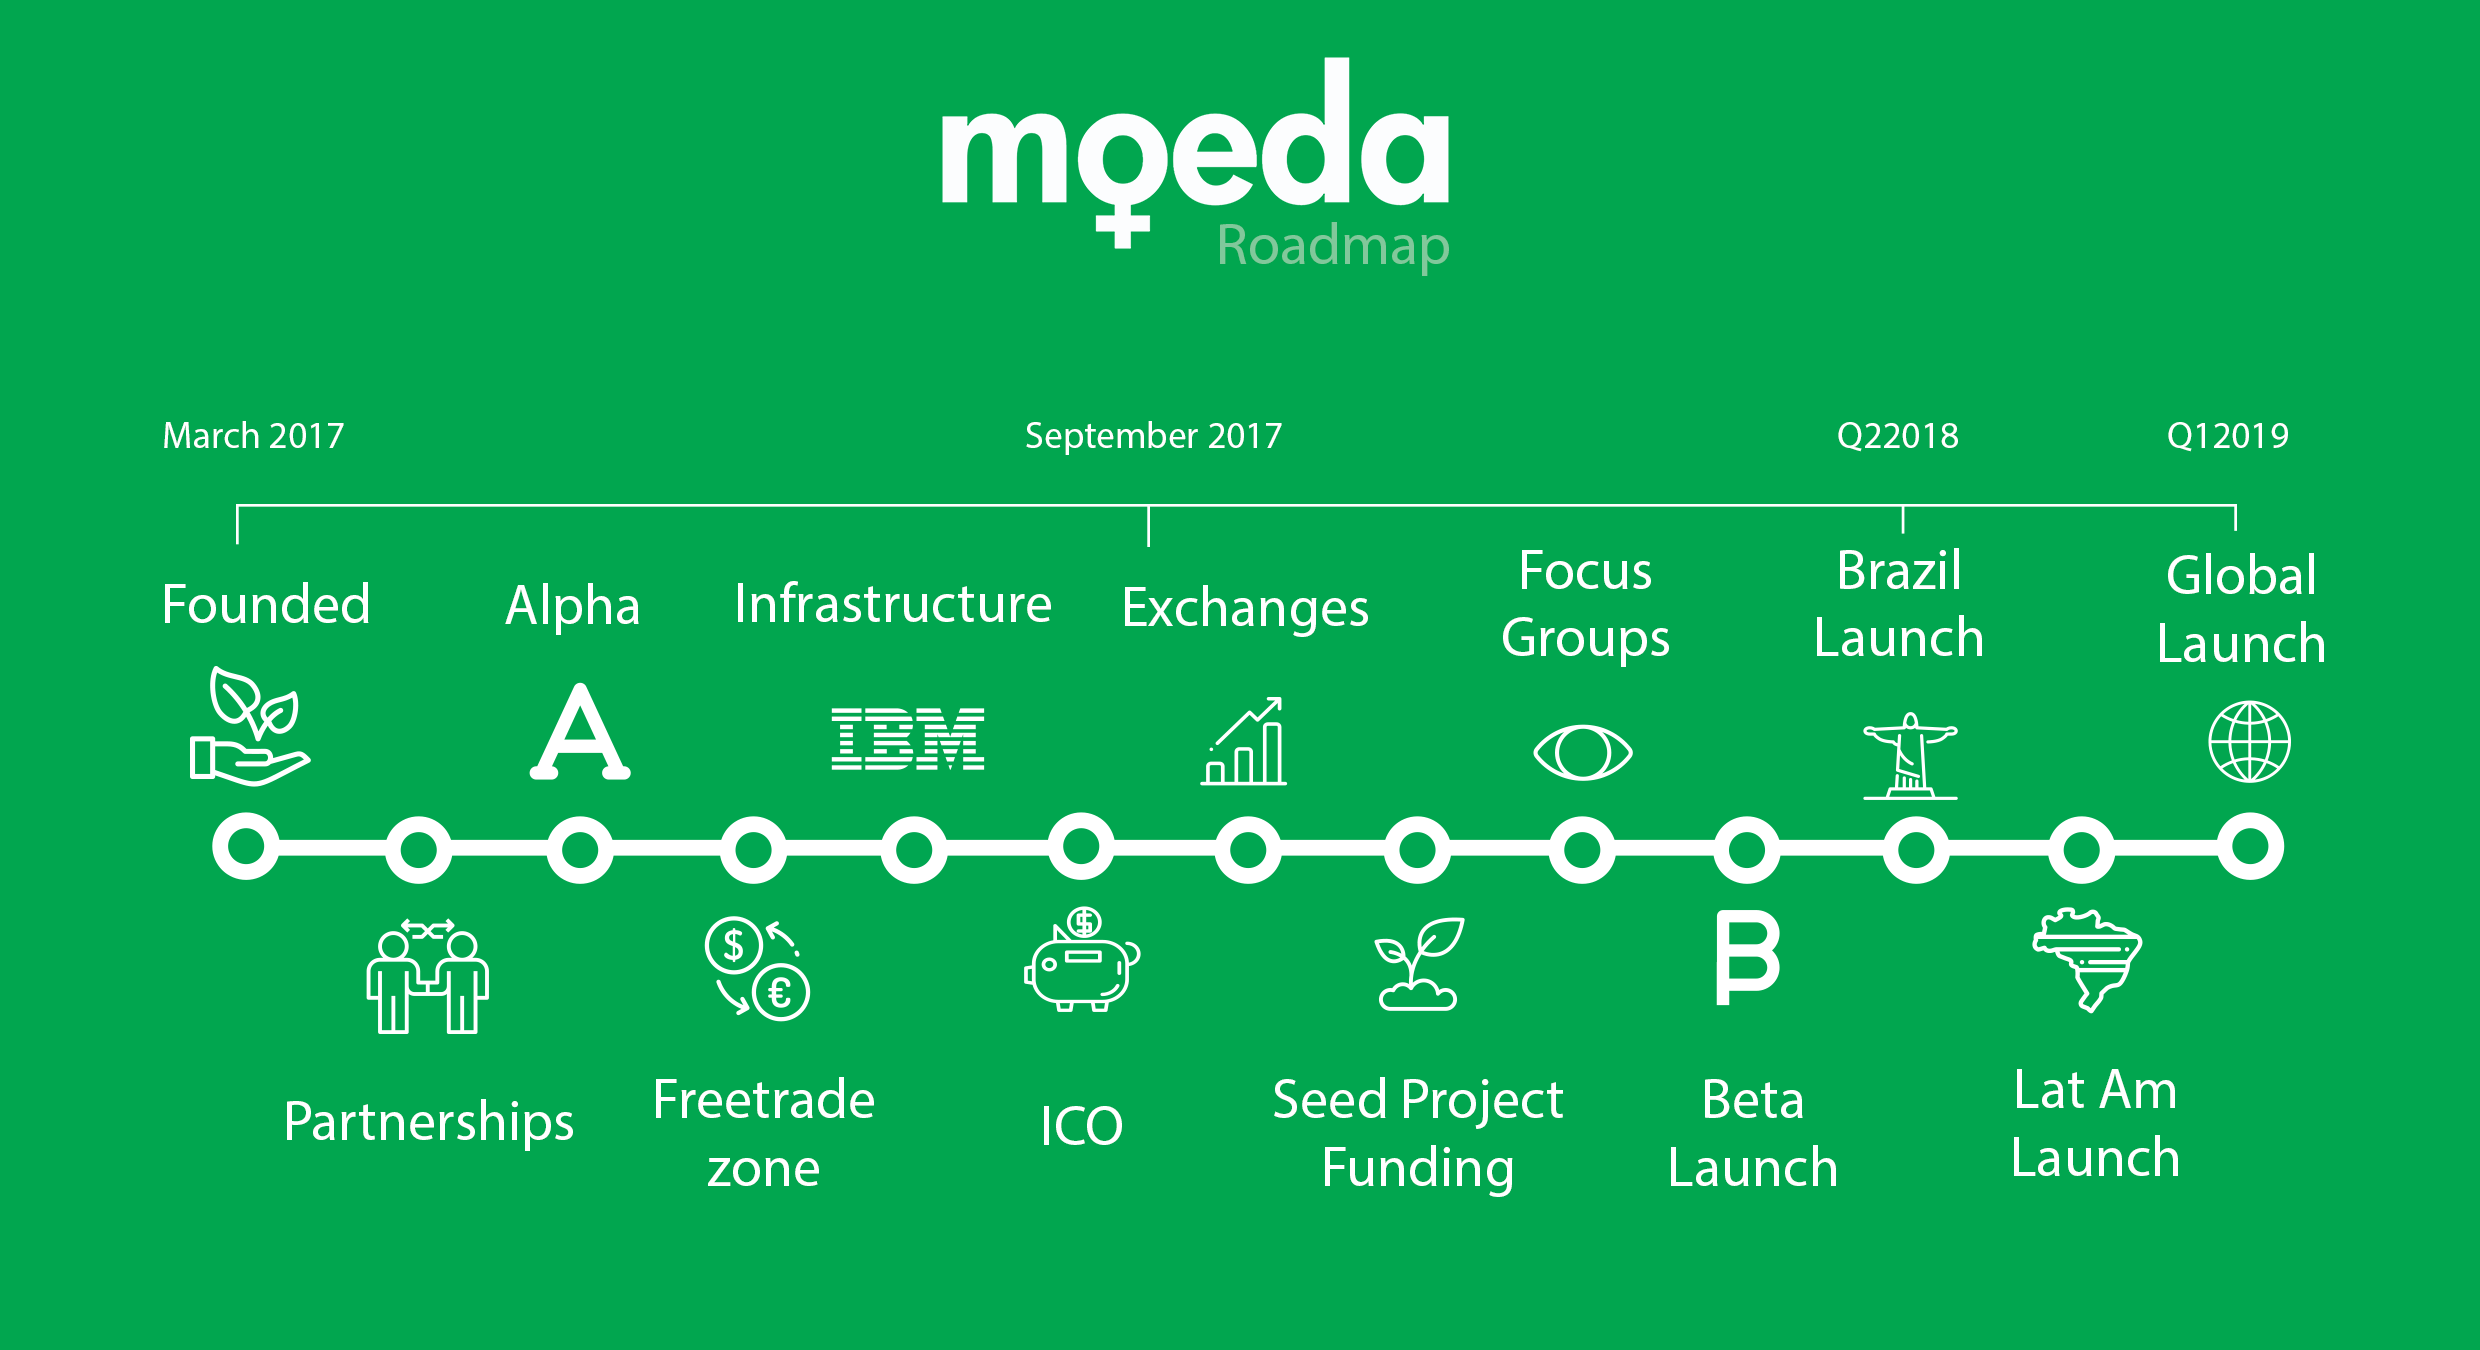
\includegraphics[width=10cm,keepaspectratio]{roadmap}
\end{figure}

\begin{figure}[h]
    \centering
    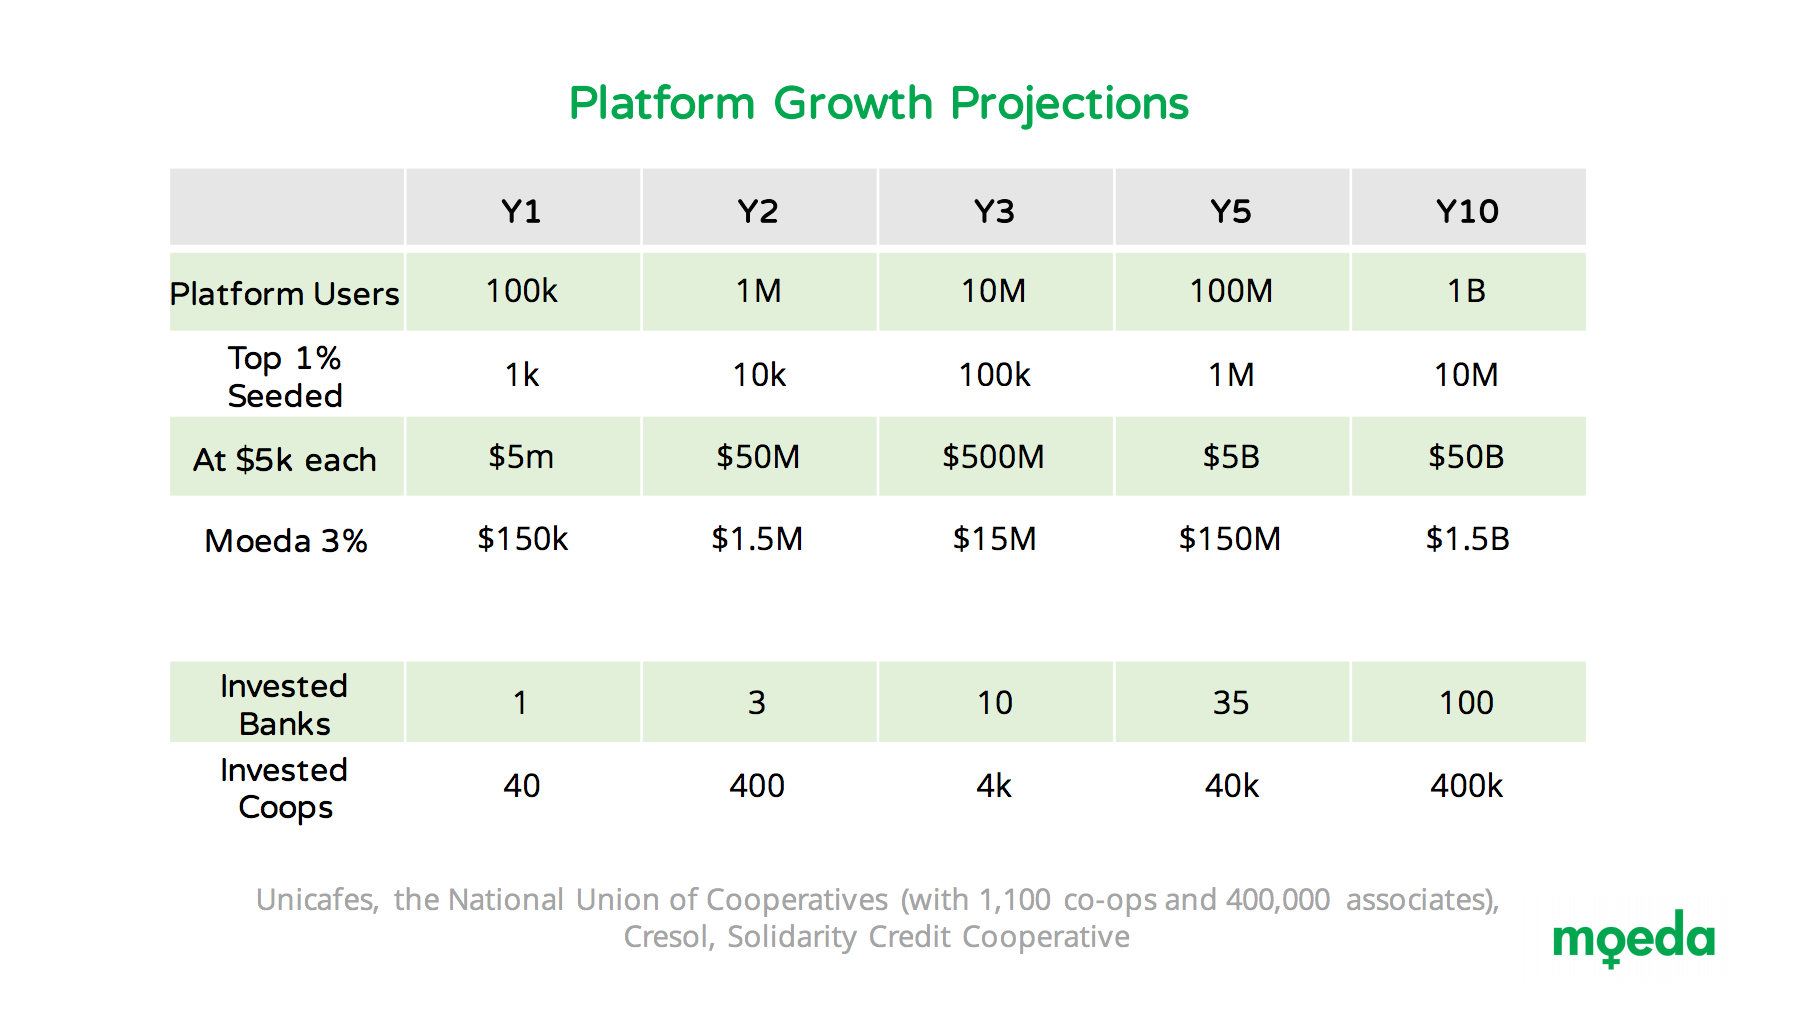
\includegraphics[width=10cm,keepaspectratio]{grow}
\end{figure}

We will we start in Brazil with 100,000 cooperative members registered on the platform that will be able to make payment transfers, remittance and loans. We plan to expand the system in 2022 to reach 1 million.
In the next 10 years MOEDA’s platform can be widely used in cities, favoring local commerce and jobs opportunity of its population, by exchanging Reais with all the Community Banks in Brazil. This can be multiplied with the adhesion of cooperatives to MOEDA, housing in each cooperative a session with the same purposes as the community banks.
The challenges of scaling impact investment in Brazil are similar to Africa, India, China, Philippines and many other developing countries. Once the model is successfully proved in Brazil we will expand quickly our solution globally.


\subsection{MDA Token details}

MOEDA (Symbol MDA) 

MDA is a ERC20 loyalty token.  A loyalty token allows investors to show their affiliation and level of support of the venture.  It does not represent equity in the company nor have any intrinsic value, therefore the value of the token should be positively correlated to the success of the project.

\subsection {MOEDA Token Utilization}

MOEDA investors will be able to access their MDA balance in the MOEDA Platform application. MOEDA users can invest MDA into MOEDA Seed Projects. MDA can be sent between users.
MOEDA users can request to land money by submitting new MOEDA Seed Project. The projects are subjected to AML/KYC MOEDA analysis.  

\section {MOEDA Revenue Model}

The MOEDA platform will be licensing the platform and its proprietary technology to banks in exchange for fees or revenue share. 

MOEDA helps the Cooperative Credit Banks originate new sustainable loans, then it syndicates or sells these loans to 3rd party investors. This process allows legal creation of the loan and transfer of funds to the borrowers based on an existing banking license. On the payment side, the depository is a collaborating Cooperative Credit Bank and all members who borrow on the platform will be onboarded as a bank member with full AML/KYC and associated accounts.

\section{ Crowd-sale of MOEDA Tokens }

MOEDA’s Initial Contribution Offering Crowd Sale, will issue loyalty tokens for donations to Green Cross Brazil during the ICO period. Loyalty tokens will be a free-floating asset.

\subsection{Green Cross Brazil}

The Green Cross Brazil is an affiliate of Green Cross International which is a non-profit founded by Mikhail Gorbachev to "respond to the combined challenges of security, poverty and environmental degradation to ensure a sustainable and secure future."

In contrast to other ICOs of which many have setup Swiss foundations to issue and hold tokens, MOEDA has partnered with the Green Cross Brazil to handle creation and distribution of tokens. Contributions to Green Cross Brazil during the ICO period will be used for the development and deployment of the MOEDA project. To this end, MOEDA has signed a services agreement to handle all of Green Cross Brazil's technology and banking services; this also includes the ability for MOEDA to charge and earn fee revenue on it's deployed platform.

\subsection {Crowd-sale Contribution Phases}

There are a maximum of 20 million tokens that will be issued.

MOEDA's european partner, Bitcoin Suisse AG company is a regulated crypto financial broker, asset manager and service provider based in Zug, Switzerland that will help MOEDA to facilitate direct donations of our tokens for BTC and FIAT out of the 9 million tokens that it holds. 

MOEDA's asian partner, ICOAGE company is a crypto financial broker based in Shanghai, China that will help MOEDA to facilitate direct donations of our tokens for ETH  out of the 2 million tokens that it holds. 

MOEDA's brazilian partner, BROOTA company is a regulated crowdfunding virtual platform based in São Paulo, Brazil that will help MOEDA to facilitate direct donations of our tokens for FIAT out of the 1.5 million tokens that it holds. 

The on-boarding of the private contribution phase via Bitcoin Suisse starts on July 18th, 2017.
The on-boarding of the private contribution phase via ICOAge starts on August 26th, 2017
The on-boarding of the private contribution phase via Broota starts on August 28th, 2017.


A \$\ 1 USD contribution in ETH will receive 1 MOEDA (MDA) token. The USD/ETH exchange rate should be updated on a daily basis.
	
More at https://moeda.in


\subsection {MOEDA Crowd-sale Contribution Token Allocation}

The ICO funding will be used to develop the platform, structure operations and logistics to technically assist borrowers and a larger part will be invested into the MOEDA revolving fund for investments into the first 100 Moeda project/loans. The operation management of the Moeda Seed Projects Program will be in partnership with UNICAFES, CRESOL, and among other credit, production and commercialization cooperative institutions.

Previous buyers of MOEDA tokens will receive a loyalty bonus on their initial outlay to compensate for realignment of the token peg. Token holders may also be given special rewards and access based on the amount and duration of tokens held. The loyalty tokens issued during the ICO will be a freely floating loyalty asset. 

MOEDA is a simple, peer-to-peer payments, peer- to-peer remittance and landing platform helping drive entrepreneurs towards their goals.

It leverages a fiat-pegged MOEDA digital token, that can travel farther and faster than physical cash ever could, granting access to micro business loans and crowdfunding, through blockchain based Android and iOS applications, empowering underbanked entrepreneurs.

The Platform will be available shortly after the ICO as they are currently in development.  

We will we start in Brazil with 100,000 cooperative members registered on the platform that will be able to make payment transfers, remittance and loans. We plan to expand the system in 2022 to reach 1 million.  


\subsection {Impact Investment}

The World Economic Forum report’s recent definition of impact investing as “an investment approach that intentionally seeks to create both financial return and positive social or environmental impact that is actively measured.” 

Moeda Seed Projects Program have the commitment to maximizing the total performance (financial and extra-financial) of the total impact investment portfolio. 
Moeda evaluates the risk that the Impact Investor is willing to carry, his tolerance for actually losing invested funds due to failed ventures/ investments, the degree to which current investments under consideration will make the overall portfolio “un-balanced” with regard to its general risk exposure or other factors that should be considered when allocating funds to a longer-term investment approach.

In addition to asset class risk, there is also thematic area risk. MOEDA offers assess to various investments and our asset classes are value-based and in alignment with the United Nations Sustainable Development Goals. The category of sustainable agriculture may have a lower risk assessment than investments in Renewable Energy. Loans to cooperatives with secured government contracts can be paid back over months, with less risk and structured as the same debt offered to an small business development fund.

\subsection {Cooperative Financial Network}

\begin{figure}[h]
    \centering
    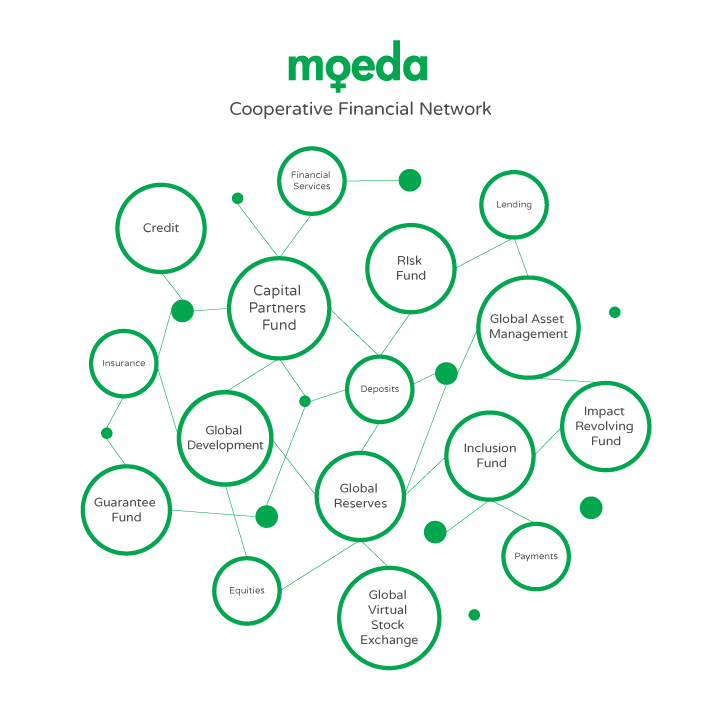
\includegraphics[width=10cm,keepaspectratio]{network}
\end{figure}

MOEDA aims to create a banking-as-a-service cooperative financial network and will treat different impact investors differently with “tailor made” risk approaches for micro-segments. 

Loans and donations to projects will be tracked transparently with a blog like format where investors can see pictures and videos of their investments in action and even discuss or give supporting words to the project. The projects themselves will be tradable blockchain assets on a future exchange to provide more liquidity and a lower cost of capital for entrepreneurs. 

At the bank level, a parallel accounting system will be implemented by Moeda which is based on a at backed blockchain system for correspondent banking and internal customer payment reconciliations to lower cost transactions. 

The long-term product vision is to create a lower cost global transparent and network of trust and cooperation like Kiva / Alipay / Paypal solution for the underbanked population of the world.


\subsection {Impact Portfolio}

The Impact Portfolio aims to grow by investing in the institutional-quality MOEDA Seed Projects and MOEDA Funds that generate competitive risk adjusted returns. 

\subsection {Impact Credit}

Will be applied for financial support of projects in the rural area, mainly those directed to government acquisitions; To support projects of families that are part of the cooperative system economy institutions (confections, handicrafts, etc.). Is a low risk portfolio designed to maintain account balances and improve liquidity.

\subsection {Impact Double Bottom Line Loans}
Elaboration and implementation of projects of community interest such as schools, health centers, affordable housing, community meeting rooms with rates of return below the market. Development and implementation of community production projects such as solar power plants, vegetable gardens and community farms, handicraft workshops, among others.

\subsection {Impact Grants and Donations}
Grants and donations will be invested in projects that do not have a financial return, but they will be managed with the same rigor as all other projects and any given bonus will be reinvested. 

\subsection {Impact Bonus}
MOEDA has designed an innovative incentive and gamified structure to increase impact strategically. We created an independent holistic credit score system with repayment estimation and a real chance to succeed at any given MOEDA Seed Project. Many people ask for money, but if they don't have the knowledge or technical support, or are not using available resources better, or are not engaging with the community, they are at a higher risk of failure. The Impact Formula helps to measure what people really truly needs are, besides financial, so we can calculate and strategically help in all levels for the success of the individual, it's community and environment.

\subsection {Integral Approach}
\textit{
"The word integral means comprehensive, inclusive, non-marginalizing, embracing. Integral approaches to any held attempt to be exactly that: to include as many perspectives, styles, and methodologies as possible within a coherent view of the topic. In a certain sense, integral approaches are “meta-paradigms,” or ways to draw together an already existing number of separate paradigms into an interrelated network of on the principles of integral research." - Ken Wilber}


The State of the World Forum (SOWF) was established in 1995 by Jim Garrison with Nobel Laureates Mikhail Gorbachev adopted the Integral approach for Politics. SOWF began as a series of annual conferences that convened hundreds of international leaders (ranging from community organizers, social activists, Heads of State, and business leaders) to explore key issues facing the globe. 

International Development organizations are aware of the value of interventions associated with the Right-Hand quadrants that focused on “development, financial management, improved communications, and policy influence. And Left-Hand quadrants that focused on “personal leadership, self-awareness, moral intelligence, and interpersonal skills.” 

\subsection {Equilibrium}

The Nash Equilibrium is a concept of game theory where the optimal outcome of a game is one where no player has an incentive to deviate from his chosen strategy after considering an opponent's choice. Overall, an individual can receive no incremental benefit from changing actions, assuming other players remain constant in their strategies. MOEDA impact metrics model is develop to prove that investing and the performance potential of capital can coexist in a sustainable way. Everybody can win, that is no trade-off between “well” while doing “good”.  

\subsection {Sentiment Analysis}

More transparency in qualifying and quantifying financial and extra-financial values more chances for everybody to win.Adam Smith in The Theory of Moral Sentiment (1759) have stated that “There is one virtue whose general rules determine with the greatest exactness every action that it requires. This virtue is justice. If I owe a man ten pounds, justice requires that I should pay him precisely ten pounds, either at the time agreed on or when he demands it. What I ought to perform, how much I ought to perform, when and where I ought to perform it, the whole nature and circumstances of the action prescribed, are all precisely fixed and determined. An holistic approach will greatly simplify the verification KYC/AML process and chances of the project to succeed. 

\section{MOEDA Seed Projects Partners}

MOEDA partners, the cooperative entities UNICAFES and CRESOL have combined 700.000 associates in more than 1.100 cooperatives and are for 30 years providing micro-loans and financial services for small agriculture families in Brazil. Under UNICAFES umbrella MOEDA is directly working with 170 Brazilian Cooperative Credit Banks and 128 Communitarian Banks to give mobile banking and access to capital for sustainable development projects. During the first year, MOEDA Seed Projects Program aims to contemplate 100.000 associates, with preference for woman, to receive MOEDA's first lines of credit.

\begin{figure}[h]
    \centering
    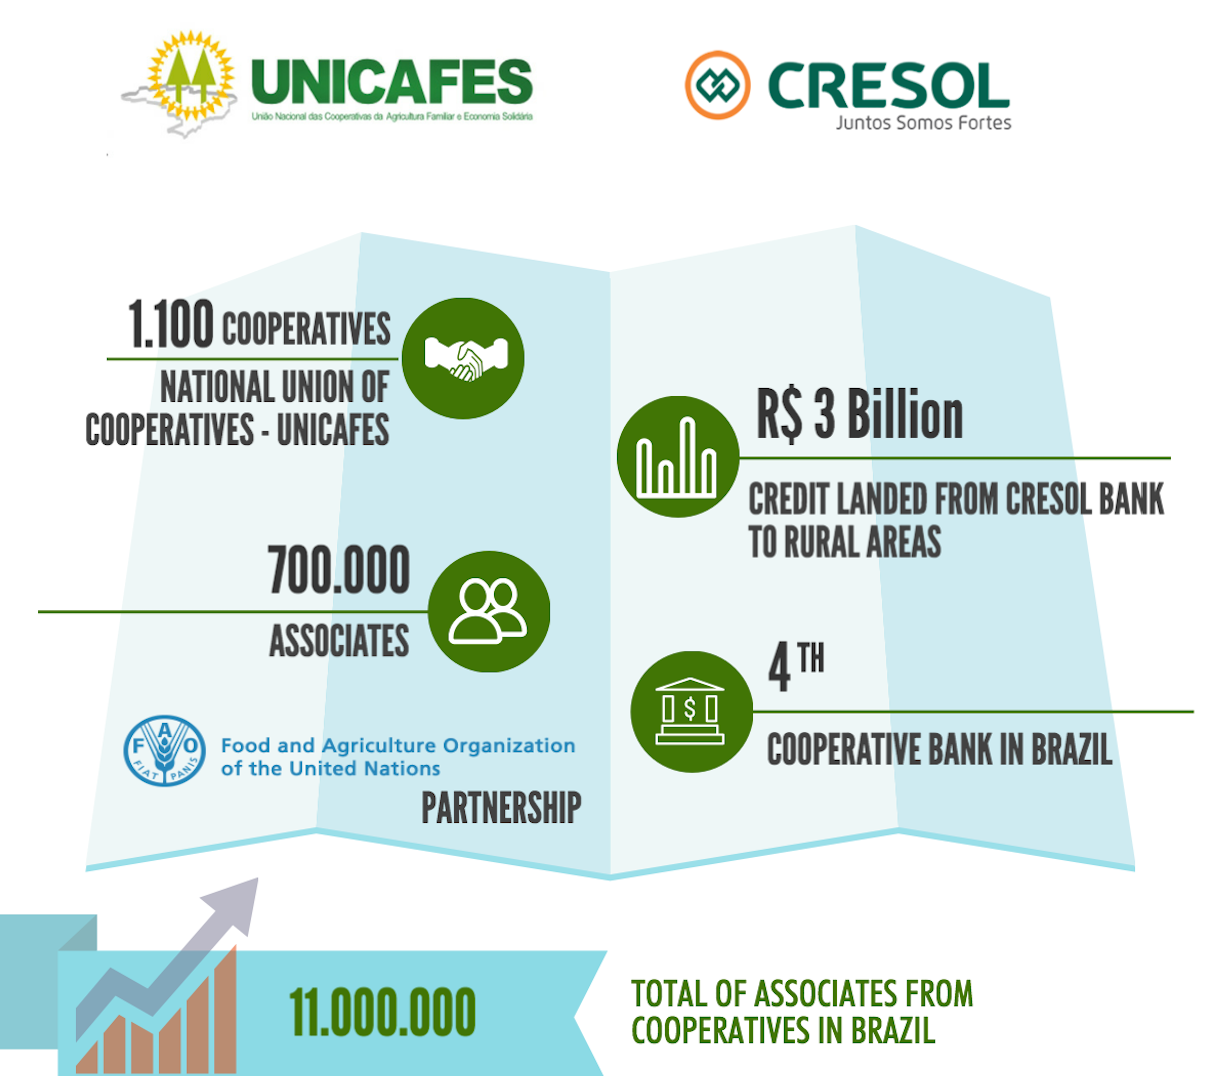
\includegraphics[width=10cm,keepaspectratio,]{bank}
    \caption{MOEDA Partners}
\end{figure}

\subsection {United Nations Sustainable Development Goals (SDGs)}

MOEDA is working towards removing three key barriers that have plagued effective public financing of the Sustainable Development Goals (SDGs):

1. Impact lenders have insufficient transparency into sustainable investments. This makes it risky to manage a large portfolio because there’s no way to see where the money is going.

2. Due to the lack of transparency, borrowers have insufficient access to capital. MOEDA gives borrowers a way to establish reputation, document project status, and to collaborate with others in the community.

3. Statistics have shown that investors have a gender bias against women-led projects, despite having historically higher success ratios and repayment rates than projects run by men. More than 40 percent of businesses registered in Latin America and the Caribbean are owned by women, according to the World Bank-IFC Enterprise survey. However, the credit gap for women-owned enterprises remains high throughout the region. Brazil has the largest gap, whereby 45 percent of women-owned SMEs identify access to finance as a major constraint in operating and growing their businesses.


\section {The Platform}

The Platform will be available shortly after the ICO as they are currently in development. 

\subsection {Technology}

Our development team is working with Native iOS/Android, PHP, Node, Golang and Haskell.


\subsection{Blockchain}

Blockchain technology is a new, powerful tool that is already shaping the future of the Internet with simple, safe and secure transactions, bringing a new wave of Economic Opportunity and Digital Innovation.

The blockchain technology facilitates the exchange of value without the need for intermediaries, enables transparent interactions of parties through a trusted and secure network that distributes certified and auditable access to data, simplifying the existing processes lowering the costs and increasing the capital efficiency.

\subsection{Ethereum}

Blockchain’s distributed ledger infrastructure had empowered Bitcoin to become a digital and easily tradable token, common used as a currency, successfully proving that distributed consensus works, but has limitations to program and customize new ideas on top of it.

MOEDA choose to work with Ethereum, that enables the development of custom programmed applications on top of the blockchain, like smart contracts, database access and storage. Ethereum Blockchain coupled with Machine Learning, Artificial Intelligence and IoT are enabling MOEDA to revolutionary innovations to building trust, immutability, transparency and traceability in transactions in both the financial system and in the real economy.

\subsection {Fees}

The fees to be charged may be differentiated for financing and loans. 3\% to 5\% of each transaction will be requested to continue improve in technology, research and development the systems that supports MOEDA and its partners network.

\subsection {Application Ranges}

 A system of application ranges can be set up with increased requirements between one and the other. (For example: ranges of up to R\$500, 500-1000, 1,000-3,000, 3,000- 5,000, 5,000-8,000 and 8,000-10,000). The borrower can start with a smaller amount of credit as she qualies and can apply for credits in larger volumes up to R\$ 10,000. It is important to note that MDA does not replace or compete with government credit lines and those established by the cooperative credit system.

\subsection {Payment Schedules for Pay Back}

Most of MOEDA applications will preferably be short-term, aiming to return to investors and to the MOEDA Program Revolving Fund. The payment deadlines must be made in accordance to each project milestone, previously defined and payment capacity of the borrower. The interest charged may follow those of Pronaf, and may refer to those charged by the Community Banks, the CRESOL System and the Cooperative Credit Systems (SICOOB, SICREDI, CONFESOL)

\subsection {Transparent Impact AML/KYC}

MOEDA has pledged to the Brazilian Central Bank, Brazilian tax authorities and regulatory bodies that it will maintain a transparent-and-compliant digital banking venture that will regularly provide information about its seed projects and other operations in the country.        

\section {The Impact Formula}

MOEDA has created a logic model to clear illustrate the path from resources to outcomes. With the Integral Equilibrium Impact Model we aim to reduce uncertainties and lowering costs, increasing our efficiency and capacity in lending and scaling and automatizing financial processes. 

\begin{figure}[h]
    \centering
    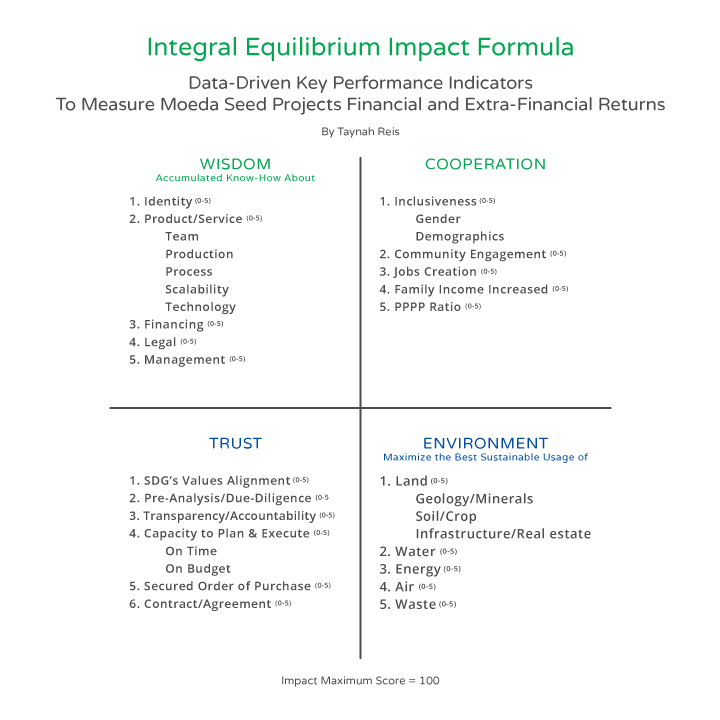
\includegraphics[width=10cm,keepaspectratio,]{moeda-formula}
    \caption{MOEDA Integral Equilibrium Impact Formula}
\end{figure}

The Key Performance Indicators to Measure MOEDA Seed Projects Financial and Extra-Financial Returns are driven by the main principles:  
•	Estimation: Conducting proper due diligence in the pre-investment analysis
•	Planning: Deriving metrics and data collection methods to monitor impact according to Integral Equilibrium Impact Formula
•	Monitoring: Measuring and analyzing impact to ensure mission alignment and performance 
•	Evaluating: Understanding post-investment impact of intervention and capital investment 
The Integral Equilibrium Impact Formula acknowledges that a personal development process, WISDOM and TRUST (I), held in place with community’s engagement and maximization of the better usage of natural resources, COOPERATION and ENVIRONMENT (We) will bring a holistic view of integrated results, aggregate outputs, outcomes, and impacts that will help with decision makers to make smart decisions on developing change. 

\subsection {WISDOM}

1.	Identity

2.	Product/ Service (People, Production, Process, Scalability, Technology) 

3.	Financing 

4.	Legal

5.	Management 


MOEDA will provide a multi-purpose digital identity and opportunities to build credit-worthiness and reputation through a holistic and integrated analysis of the individual Impact Score.
In countries like Brazil, where corruption is rampant, most of information still resides in either paper records or in outdated proprietary data bases, blockchain-enabled registries are a reliable alternative to current registries.

MOEDA will support the cooperatives, enterprises and participants of MOEDA Seed Projects in the areas of analysis, planning, production, processing, industrialization and commercialization of their services and projects with qualified professionals and technicians to guarantee its successful execution. 

\subsection {TRUST}

1.	SDG’s Values Alignment 

2.	Pre-analysis/ due-diligence

3.	Accountability and Transparency 

4.	Capacity to Plan and Execute (On Time, On Budget)

5.	Secured Order of Purchase Contract/Agreement 

We believe that MOEDA will create a global network of trust and the resulting map of outputs and outcomes from the Integral Equilibrium Impact logic model can be used to identify targets upon which incentives systems, fair interest rates, a new economy sustainable model can be designed. 

By aligning MOEDA model of incentives with the United Nations 17 Sustainable Development Goals(SDGs) we aim to create a shared, world-wide, cooperative effort where everyone is invited, has a role, and participates. The SDGs are a set of high-level goals, each grounded in a series of underlying performance indicators designed for integration and participation at every level of society and industry across the globe. Where the Millennium Development Goals largely failed to engage the world (because they were pointed at governments, not people) the Sustainable Development Goals have been translated into performance guides for businesses, curricula for schools, games, activities, workshops, and on and on. They were designed with a diverse set of on-ramps, to be a common language and measurement system for everyone.

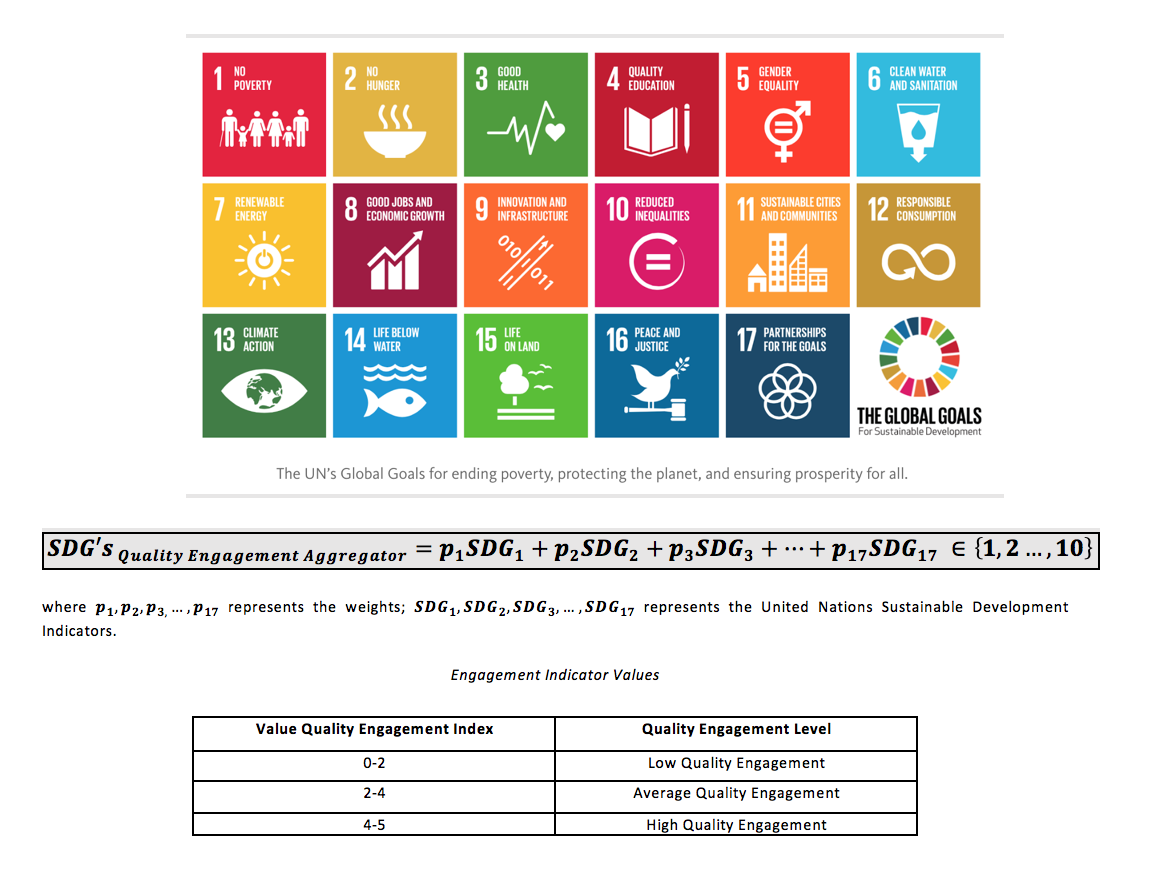
\includegraphics[width=10cm,keepaspectratio]{sdgs}

MOEDA will measure and qualify the index of engagement on each of the 17 SDGs for every MOEDA Seed Project. 

Investors can search and explore Projects by SDGs as well.

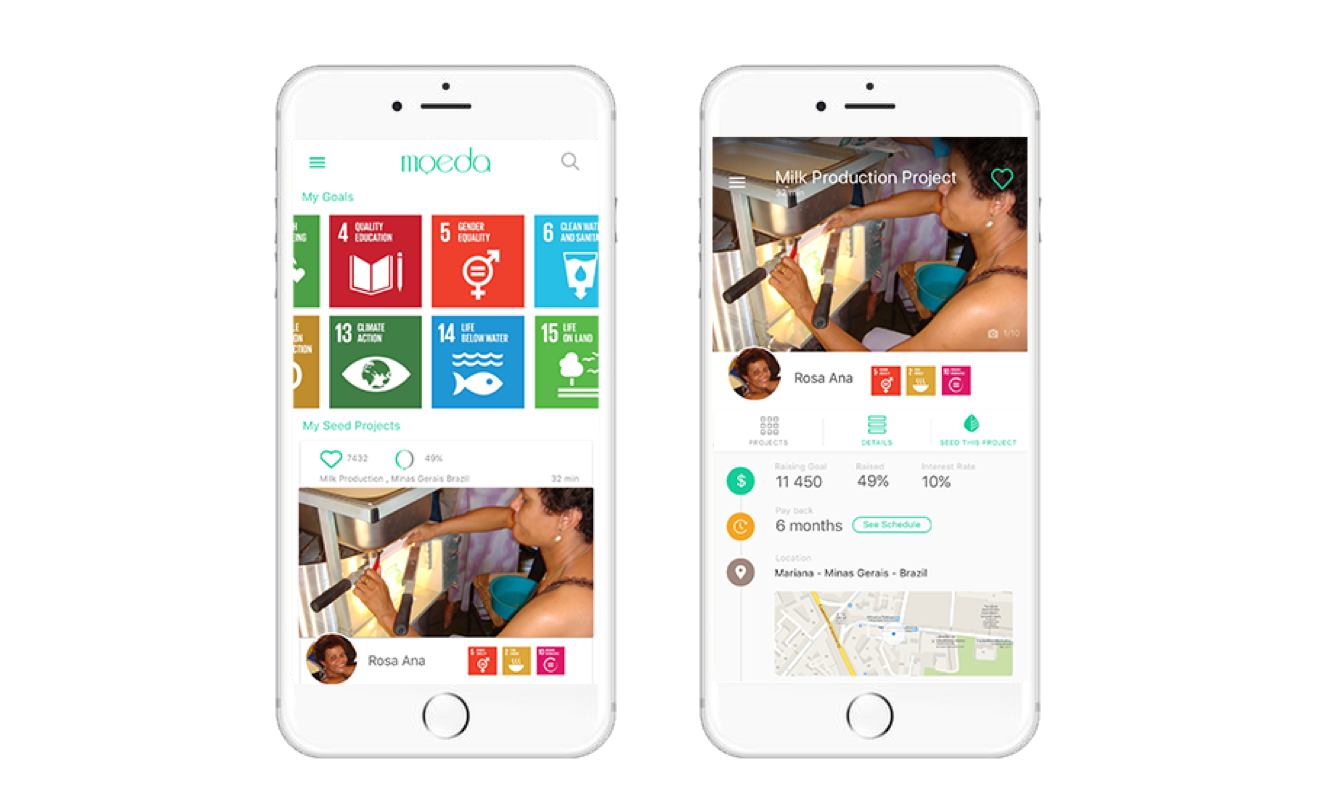
\includegraphics[width=10cm,keepaspectratio]{projects}

MOEDA provides impact investors a platform to communicate with the borrower to understand their path to intended impact. Investors can also identify areas where further due diligence on impact should be undertaken. The App is a simple way for better visualization of the impact results created for audiences that may not be familiar with sophisticated impact measurement methodologies. Output measures can provide a pulse on the operational aspects of the borrower, and can be useful as a management tool for day-to-day monitoring. 


\subsection {COOPERATION}

1.	Inclusiveness (Gender/Demographics) 
2.	Community Engagement 
3.	Jobs Creation
4.	Family Income Increased 
5.	PPPP Ratio

MOEDA Seed Projects when implemented and managed properly,  can deliver a real benefit to communities increasing savings, investment and empowering individuals to build small businesses. The platform can increase transparency in the accountability, reducing the error and fraud in government-mediated services to citizens and businesses. 


\subsection {ENVIRONMENT}

Maximize the best usage of:
1.	Land (Crop, Minerals) 
2.	Water
3.	Energy
4.	Air
5.	Waste

The quantity of resources we use and our impact on the environment effectively depend on three main factors:

Population: how many of us there are consuming resources and creating waste 

Consumption: the average amount of goods and services we each use 

Technology: how inefficiently/harmfully we produce these goods and services 

By developing the metrics to empower a trusted decision information infrastructure, MOEDA aims to create a reliable mechanism for measurement, reporting, and verification that will enable large financial flows to decarbonize the global economy, capture the massive energy efficiency opportunity, expand and conserve global carbon sinks.

\section {Future States}

\subsection {IoT and AI Integrations}

Blockchain’s smart contracts can provide smart trade finance services leveraging IoT to tag their claims on physical assets, making them trackable and traceable. All documentation relating to a particular asset to be traded can be digitized and carried on the blockchain  including ownership, warranties, inspection certification, provenance, insurance, replacement dates, approvals, significantly increasing data availability and integrity, reducing paperwork handling, storage and loss, and other process improvements related to that documentation. 

IoT and AI can have great impact on risk mitigation strategies for MOEDA as it would allow for better portfolio management, allowing a true decentralized and shared economy to blossom.

This represents a massive opportunity to stream-line trade finance processes, cut operating costs and reduce losses by better underwriting the trade finance risk through improved data analysis of exposures to serve the current latent demand, particularly in developing countries. 




\end{document}